\documentclass[tikz, border=5mm]{standalone}
\usepackage{tikz}
\usetikzlibrary{shapes.geometric, arrows.meta, positioning}

\begin{document}
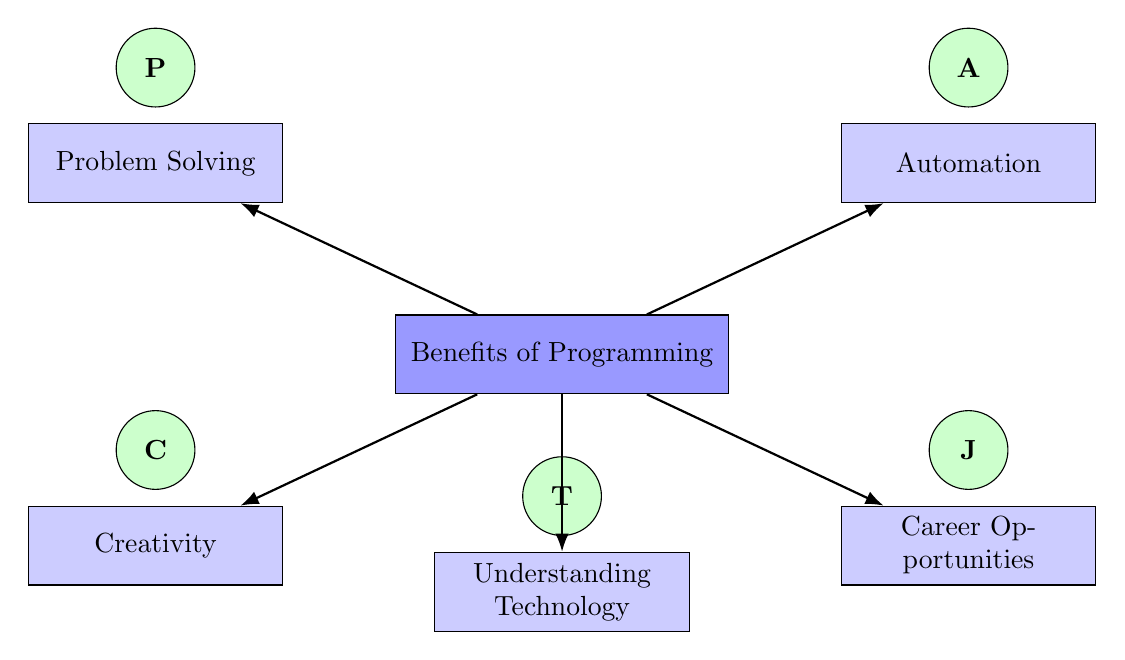
\begin{tikzpicture}[
    node distance=2cm, % Increased node distance for better spacing
    box/.style={rectangle, draw, fill=blue!20, text width=3cm, text centered, minimum height=1cm},
    icon/.style={circle, draw, fill=green!20, minimum size=1cm, inner sep=0pt, font=\bfseries},
    arrow/.style={-Latex, thick}
]

% Central node
\node (center) at (0,0) [box, fill=blue!40, text width=4cm] {Benefits of Programming};

% Benefit nodes arranged in a square
\node (problem_solving) [box, above left=of center] {Problem Solving};
\node (icon_ps) [icon, above=2mm of problem_solving] {P};

\node (automation) [box, above right=of center] {Automation};
\node (icon_auto) [icon, above=2mm of automation] {A};

\node (creativity) [box, below left=of center] {Creativity};
\node (icon_creat) [icon, above=2mm of creativity] {C};

\node (career) [box, below right=of center] {Career Opportunities};
\node (icon_career) [icon, above=2mm of career] {J};

\node (understanding) [box, below=2cm of center] {Understanding Technology}; % Keep this below center
\node (icon_under) [icon, above=2mm of understanding] {T};

% Connections
\draw [arrow] (center) -- (problem_solving);
\draw [arrow] (center) -- (automation);
\draw [arrow] (center) -- (creativity);
\draw [arrow] (center) -- (career);
\draw [arrow] (center) -- (understanding);

\end{tikzpicture}
\end{document}
